\epigraph{\textit{Logic is the foundation of the certainty of all the Knowledge we acquire.}}{-- \textup{Leonhard Euler}}

As we have seen thus far, this thesis' main goal is to create a tool capable of generating subsets out of a Knowledge graph. In this chapter, we will explore the possibility of implementing the Pregel framework in Rust, as well as following a novel approach for solving the problem of validating a Knowledge graph.

\section{Pregel-rs}

The \texttt{pregel-rs} library is a Rust fork of the original Pregel framework that we have already discussed in chapter \ref{chapter:theory}. This library is available on GitHub\footnote{\url{https://github.com/angelip2303/pregel-rs}}.

\subsection{Design}

So far, we have discussed the Pregel framework. However, for us to implement it, we need to make certain design decisions. This section will outline the compromises we have made to successfully implement the Pregel model in Rust.

First and foremost, it should be acknowledged that when transitioning from the Scala-based solution to the Rust-based one, we were fully aware that building the solution on top of existing projects would not be feasible. This stems from the fact that Rust, being a relatively new language, is not as mature as Java. Consequently, certain features would need to be developed from scratch. Thus, we started the development of the Pregel library, which will be utilized to implement the subgraph matching algorithm.

It is important to note that we have deliberately separated the framework from the algorithm implementation addressed in this thesis. This decision was made to maximize the framework's flexibility. By adopting this approach, not only can we utilize the framework in other projects, but we can also extend its capabilities to support additional features. To put an example, we have successfully incorporated the \textit{PageRank} algorithm into the framework as an additional feature to demonstrate its versatility. In the following sections, we will discuss the design and implementation details of the Pregel library.

\label{section:pregel-rs}
\subsubsection{The \texttt{pregel-rs} library}

Recall that Rust is heavily oriented to be executed in single machines. This means that we won't use the Pregel framework to process graphs in a distributed manner. Instead, we will use it to process graphs in a \textit{centralized system}. Back when the Pregel framework was introduced, the hardware resources available for single-node systems were limited. However, nowadays, we can leverage the benefits of multi-core processors to process graphs in a centralized manner. Thus we will make use of techniques such as \textit{multi-threading} to process graphs in a single machine. Note that the creation of the \texttt{wd2duckdb} tool was motivated by the idea of trying to make it fit the whole graph in memory. To put it into perspective, as of 2023, we, as customers, can purchase a memory module with a capacity of 128 GB with a total cost of $\$269.90$. However, this was not the case back in 2010, when the Pregel framework was introduced. Thus, we are hopeful that we can create a Pregel-like framework that instead of processing graphs in a distributed manner, can make use of the hardware resources available in a single machine; this is, a \textit{multi-threaded Pregel}. Recall what we have mentioned in section \ref{section:rust} about the way \textit{concurrency and parallelism} are implemented in Rust.

The idea then is to optimize the use of memory as much as we can to process graphs in a single machine. As a comparison, the size of the Wikidata JSON dump created as of August the $21^{th}$ 2017 is $16.94 GB$ compressed ($224.42 GB$ uncompressed), while the \texttt{.duckdb} database file created by the \texttt{wd2duckdb} tool is $9.38 GB$. This means that we can fit the whole graph in memory, and hence, we can fit the graph in a single machine. However, we need to be careful when processing the graph, as we can easily run out of memory. To avoid this, we will make use of the \textit{lazy evaluation} technique. This mechanism will allow us to process the graph in a \textit{streaming} manner, which will reduce the memory footprint of the application. More into this will be discussed later on.

Firstly, we are describing the series of steps that the Pregel framework follows to process a graph. This sequence is depicted in figure \ref{fig:sequence}. The execution starts by sending the initial messages to the vertices at iteration 0. Then, the first -- actual -- superstep begins. This loop will last until the current iteration is greater than the threshold set at the creation of the Pregel instance. At each iteration, the vertices will send messages to their neighbors, provided the given direction, and subsequently, they may receive messages sent from other nodes. Moving forward, an aggregation function is applied, and the vertices are updated accordingly. Finally, the iteration counter is incremented, and the next iteration starts until the threshold is reached.

\begin{figure}[ht]
    \centering
    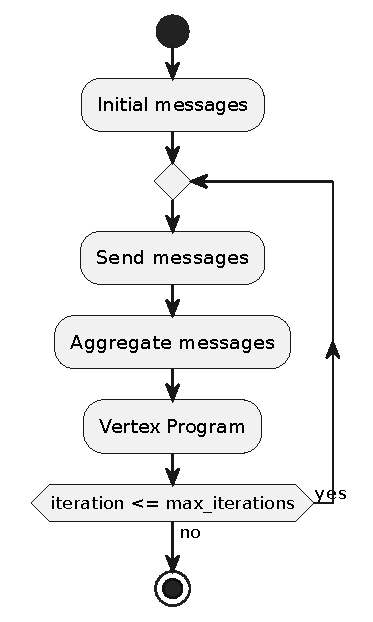
\includegraphics[width=0.4\textwidth]{diagrams/11-1_pregel.pdf}
    \caption{The Pregel framework as implemented in \texttt{pregel-rs}}
    \label{fig:sequence}
\end{figure}

As you can observe, the described process is far from being complex. Thus, we can agree that the Pregel framework is a simple abstraction for graph processing. However, this simplicity is what makes the Pregel paradigm so powerful. By abstracting the underlying model, we can focus on the problem at hand, rather than the implementation details of the framework. By doing so, we can focus on the implementation of the \textit{subgraph matching algorithm}, rather than the implementation details of the Pregel model itself. Now that we have a better understanding of what we are trying to build, we can move forward and discuss some of the design decisions we have made.

\subsubsection{The Builder pattern}

In Rust, there is no direct support for constructors. Instead, the convention is to use an associated function called \texttt{new} that returns an instance of the \texttt{struct}. However, this restricts the creation of objects to only one possible representation, since multiple functions cannot have the same identifier. Unlike Java, where we can have multiple constructors with the same name, as long as they have different parameters. To overcome this limitation and enable the creation of different representations of the same object, we can utilize the \textit{Builder pattern}.

\begin{figure}[ht]
    \centering
    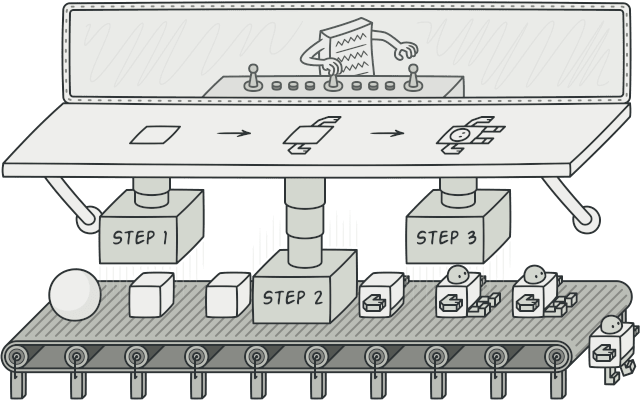
\includegraphics[width=0.66\textwidth]{diagrams/11-2_builder.png}
    \caption[Diagram showing the idea behind the \textit{Builder pattern}]{Diagram showing the idea behind the \textit{Builder pattern}\footnotemark}
\end{figure}
\footnotetext{\url{https://refactoring.guru/design-patterns/builder}}

This is a creational design pattern that allows us to decouple the construction of a complex object from its functionality. By separating the construction process, we gain the flexibility to create diverse representations of the object itself. This pattern effectively resolves the issue of dealing with constructors that have an excessive number of parameters and also addresses Rust's limitation of having only one \texttt{new} function per \texttt{struct}. It also allows us to \textit{create} objects in a -- somewhat -- functional manner, which is a common practice in Rust. As a last remark, the \textit{Builder pattern} allows us to create a default representation of the object, which is useful when we want to create a default configuration of it, and then modify it accordingly. What's more, it allows us to build objects in such a manner that some configuration aspects are optional. In the example below we can observe the creation of a Pregel instance using the Builder pattern. What we are doing is creating a default configuration of the Pregel instance, by calling the \textit{new} function, passing the \texttt{GraphFrame} object, which is the only required parameter. Then, by subsequent calls to the builder methods we can modify the object's representation. As an example, we are setting the maximum number of iterations to 4. Finally, we are calling the \texttt{build} function which will return the -- actual -- Pregel instance with the desired representation. Note that, in this case, what we are building is the so-called \textit{PageRank} algorithm\footnote{\url{https://github.com/angelip2303/pregel-rs/blob/main/examples/pagerank.rs}}, which is a well-known algorithm for ranking web pages.

\begin{code}[Creating a Pregel instance using the Builder pattern]
    \inputminted{rust}{code/listings/11-3_pagerank.rs}
\end{code}

\subsection{Implementation}

We will now discuss the implementation details of the Pregel library that we have just described. Recall that we are willing to create a tool that is implemented on top of a DataFrame API, as we want to leverage the benefits of this abstraction that we have already discussed in chapter \ref{chapter:refactoring}. Thus, we will now comment on the implementation details of the Pregel library.

\subsubsection{The \texttt{GraphFrame} struct}

The first step is to create a representation of the graph that we are going to process. To do so, we have created the \texttt{GraphFrame} struct. This struct is a wrapper around the \texttt{pola-rs} \texttt{DataFrame} library, which is the equivalent in Rust to Apache Spark's \texttt{DataFrame API}, as we have seen in chapter \ref{chapter:analysis}. This \texttt{struct} is responsible for storing the graph's vertices and edges, as well as extending its basic functionality to support some useful operations. For example, we have implemented the \texttt{from\_edges} function, which is responsible for creating a \texttt{GraphFrame} instance from a set of edges. This function is useful since it allows us the creation of the \texttt{GraphFrame} from the entities that we have extracted from the Wikidata JSON dump in chapter \ref{chapter:wd2duckdb}.

As we have introduced in section \ref{section:pregel-rs}, the way we are implementing the \texttt{pregel-rs} library is through a \texttt{Lazy API}. What we mean by this is that operations are not computed until we explicitly specify so. This has a great advantage when working with large datasets, as we can \textit{optimize} the query we are building. Let me clarify this. When we evaluate functions more traditionally; that is, \textit{eager evaluation}, expressions are computed as soon as they are defined. This means that, if we have a chain of operations, each operation will be computed as they appear in the code. However, things are different when using \textit{lazy evaluation}, as expressions are not computed until we need the actual result of the evaluation. This allows \textit{query engines} to optimize the query, by reordering the operations in such a way that the number of actual computations is reduced. In the example below, we can observe how operations are not computed until we call the \texttt{collect} function, in line 20, which is the one that triggers the computation. Note that we can use this technique as we call the \texttt{lazy} function before referring to the computations we want to perform over the dataset. This has another enormous advantage, which is that we can \texttt{clone} the objects that we are working with, without having to worry about the performance implications of doing so. This is because, as we have mentioned, the actual computation is not yet performed, and hence, we are just \texttt{cloning} the \textit{query plan}\footnote{\url{https://stackoverflow.com/questions/72320911/how-to-avoid-deep-copy-when-using-groupby-in-polars-rust}}.

\begin{code}[GraphFrame implementation in \texttt{pregel-rs}]
    \inputminted{rust}{code/listings/11-1_graph.rs}
\end{code}

\subsubsection{The \texttt{Pregel} framework}

Thus far, quite a lot has been said about different \texttt{structs} and features that are helpful for the implementation of the Pregel algorithm. However, we have not yet discussed the actual algorithm. In this section, we will comment on the implementation details of the Pregel model in Rust, which is the core of the \texttt{pregel-rs} library. Recall diagram \ref{fig:sequence} where we showed the different steps that are involved in the Pregel framework.

First, we will start by describing the \texttt{initial\_message} step\footnote{\url{https://github.com/angelip2303/pregel-rs/blob/main/src/pregel.rs\#L764}}. Note that, at this point, we are working with a Graph containing a bunch of vertices and edges. No operation has been performed yet. Thus, we need to create -- at least -- one extra column for the messages to be sent, back and forth. What's more, we have to initialize that column to a certain value, which is specified by the user during the configuration of the Pregel instance. This is done by selecting all the columns in the DataFrame, and then, selecting also the result of applying the \texttt{initial\_message} column. Regarding the point in time at which we \texttt{collect} the results of the computation, this will be performed at the end of each \textit{superstep}. This means that, at the end of each iteration, we will get a DataFrame containing the vertices having the different operations evaluated. By doing this, we ensure that at the beginning of each iteration, the vertices are in the state that we expect them to be. Recall that in the Pregel model, the \texttt{initial\_message} step is known as the \textit{superstep 0}, and hence, we will \texttt{collect} the results of the computation.

Note that another optimization is introduced here, which is the use of the \texttt{Streaming API}. With the combination of the \texttt{lazy} and \texttt{streaming} APIs, we can perform the computation in such a way that we are not going to load the whole dataset into memory, but it is going to be processed in chunks. This is a great advantage when working with large datasets, as we can avoid the \textit{out of memory} errors that we would otherwise encounter. Another advantage is that we can work with datasets that are larger than RAM. See the code below for a more detailed explanation.

\begin{code}[Initial step as implemented in \texttt{pregel-rs}]
    \inputminted{rust}{code/listings/11-4_initial.rs}
\end{code}

To go a step further, we will now describe the main loop of the Pregel algorithm. This is, we now have all the vertices and edges of the Graph annotated with an extra column, namely, the \texttt{vertex\_column}. Thus, it is time for the \textit{superstep 1} to begin. This is divided into three main pieces. The first step is to send the messages in the appropriate direction. Just after that, those messages are aggregated. Lastly, the vertices are updated accordingly. For us to perform the first step, we must apply the \texttt{send\_message} function to the whole graph. After that, the messages are going to be sent in the given direction. Note that, one node may have many neighbors. Hence, we must \textit{aggregate} the messages into a single one. This is done by applying the \texttt{aggregate\_messages} function. In the case of the \texttt{pregel-rs} library, we are using a \texttt{groupby} context. The code below shows how it is implemented\footnote{\url{https://github.com/angelip2303/pregel-rs/blob/main/src/pregel.rs\#L829}}. Note that some simplifications have been made, but the idea is the same.

\begin{code}[Messages step as implemented in \texttt{pregel-rs}]
    \inputminted{rust}{code/listings/11-5_msgs.rs}
\end{code}

Moving on, now that we have the messages sent and properly aggregated, it is time to update the vertices. What we mean by this is that according to the Pregel model, the vertices may need to be modified to reflect their new state due to the messages they have received. This is done by applying the \texttt{v\_prog} function to the graph. For us to achieve so, we need to join the vertices with the messages sent. In our case, an \textit{outer join} is performed, as we want to produce a \texttt{DataFrame} that contains all the rows from both \texttt{DataFrames}. That is, we don't want to lose any of the information. The only issue regarding this \textit{join strategy} is that it may populate the resulting \texttt{DataFrame} with \texttt{NULL} values if the join key does not exist in the source \texttt{DataFrame}. However, in the case of our solution, we know, we are working with \textit{strongly connected graphs}, as is the case of Knowledge graphs. The code below shows how it is implemented in \texttt{pregel-rs}\footnote{\url{https://github.com/angelip2303/pregel-rs/blob/main/src/pregel.rs\#L839}}. This is the last step of the \textit{superstep 1}. Note that, at this point, we have already performed the first iteration of the Pregel algorithm. Thus, we need to get ready for the next iteration.

\begin{code}[Vertex Program step as implemented in \texttt{pregel-rs}]
    \inputminted{rust}{code/listings/11-6_vprog.rs}
\end{code}

As we have already mentioned, the last part of each \textit{superstep} is in charge of ensuring the correct execution of the algorithm. This is, we need to make sure that the operations performed won't affect the \textit{integrity} and \textit{consistency} of the algorithm. For us to do so, we are going to \textit{materiallize} the results of the computation and increment the iteration counter. The code below shows how it is implemented in \texttt{pregel-rs}\footnote{\url{https://github.com/angelip2303/pregel-rs/blob/main/src/pregel.rs\#L854}}.

\begin{code}[Getting ready for the next iteration of the Pregel algorithm]
    \inputminted{rust}{code/listings/11-7_collect.rs}
\end{code}

For more information on how the Pregel model works, take a look at the appendix \ref{appendix:trace} of this thesis where a trace of the execution of a \textit{PageRank} algorithm implemented on top of the library is shown.

\section{PSchema-rs}

\subsection{The algorithm in a nutshell}

In this section, we will describe the algorithm that we are using to validate the Knowledge graph. The idea is to transform the given set of rules, \texttt{Shape} \texttt{Expression}, into a tree that is going to be traversed by the Pregel model that we have just described, namely, the subgraph matching algorithm. This idea takes inspiration from the \textit{Distributed subgraph matching algorithm} presented in \cite{Xu2019}; however, several modifications are introduced due to the requirements of our project.

\subsubsection{The \texttt{Shape} \texttt{Expression} tree}

Given a \texttt{Shape} \texttt{Expression} schema $\mathcal{S}$, we assume that it is a collection of labeled \texttt{Shape} \texttt{Expressions} that describe an RDF graph in terms of three main syntactic components\footnote{\url{https://shex.io/shex-primer/}}: \texttt{Triple Constraints}, \texttt{Shape References} and \texttt{Groupings of Triple Constraints}. The former is a triple pattern that describes a predicate-subject statement matched by the sub-setting algorithm. The second is another triple constraint where the subject is a reference to a \texttt{Shape}. The latter is a grouping of several of those constraints. The \texttt{Shape} \texttt{Expression} schema is going to be transformed into a tree, called \texttt{Shape} \texttt{Expression} tree, that is going to be traversed by the validation algorithm. This tree is going to be built recursively, and it is going to be traversed in a bottom-up fashion. This means that we are going to start by validating the leaves and then we are going to build the internal nodes, that is, the tree is going to be traversed in a \textit{reverse level order} fashion, as we need the children to be validated first for us to work with their parents. This is going to be done by an \texttt{iterator} that we will describe later on.

Putting this all together, \texttt{Shape} \texttt{Expressions} can be divided into two main categories according to the tree that they are going to generate, namely, \textit{unary} and \textit{n-ary} components. The former is going to generate a tree with a single node labeled with the identifier of the \texttt{Triple Constraint}, or, a single node with a single child in the case of a \texttt{Shape Reference}. The latter is going to generate a tree with a single node labeled with the identifier of the \texttt{Shape} that wraps the \texttt{Grouping} and with $n$ children. For each child, we are going to build their corresponding \texttt{Shape} \texttt{Expression} tree. This is going to be done recursively. For more information, see the \texttt{Shape} \texttt{Expression} tree definition.

\begin{definition}
    The \texttt{Shape} \texttt{Expression} tree $T$ is defined as follows. Having $\mathcal{S}$ a \texttt{Shape}, two main cases are possible:

    \begin{itemize}
        \itemsep0.5em
        \item If $\mathcal{S}$ is a \textit{unary} component, two cases are possible:
              \begin{itemize}
                  \itemsep0.25em
                  \item If $\mathcal{S}$ is a \texttt{Triple} \texttt{Constraint}, then $\mathcal{T}$ is a tree with a single node labeled with the identifier of the \texttt{Shape}.
                  \item If $\mathcal{S}$ is a \texttt{Shape Reference}, then $\mathcal{T}$ is a tree with a single node labeled with the identifier of the $\mathcal{S}$ shape and with a single child, $\mathcal{T}_1$, which is the \texttt{Shape} \texttt{Expression} tree of $\mathcal{S}_1$.
              \end{itemize}
        \item If $\mathcal{S}$ is a \textit{n-ary} component, one case is possible:
              \begin{itemize}
                  \itemsep0.25em
                  \item If $\mathcal{S}$ wraps a group of \texttt{Shapes}, then $\mathcal{T}$ is a tree with a single node labeled with the identifier of the $\mathcal{S}$ shape and with $n$ children,$\{\mathcal{T}_1, \mathcal{T}_2, ..., \mathcal{T}_n\}$, which are the \texttt{Shape} \texttt{Expression} trees of $\{\mathcal{S}_1, \mathcal{S}_2, ..., \mathcal{S}_n\}$, respectively.
              \end{itemize}
    \end{itemize}

    Note that the \texttt{Shape} \texttt{Expression} tree is going to be built recursively. Hence, the base case is the first item of this definition, and the recursive cases are the other two. In this manner, by chaining recursive cases, we can build a tree with an arbitrary depth.
\end{definition}

Following into this definition, we have only implemented part of the \texttt{Shape} \texttt{Expression} model as it is out of the scope of the project; recall, we are mainly interested in the \texttt{Triple} \texttt{Constraint} component. However, it is easy to extend the implementation to support the other components. For more information, see the \texttt{Shape} \texttt{Expression} model implementation in \texttt{pschema-rs}\footnote{\url{https://github.com/angelip2303/pschema-rs/issues/1}}.

\begin{table}[ht]
    \centering
    \begin{tabular}{|l|c|l|c|}
        \hline
        \rowcolor[HTML]{EFEFEF}
        \multicolumn{1}{|c|}{\cellcolor[HTML]{EFEFEF}\textbf{Feature}} & \textbf{Supported}         & \multicolumn{1}{c|}{\cellcolor[HTML]{EFEFEF}\textbf{PSchema Representation}} & \multicolumn{1}{c|}{\cellcolor[HTML]{EFEFEF}\textbf{Tree Category}} \\ \hline
        Triple and Node Constraints                                    & {\color[HTML]{009901} Yes} & \texttt{Triple Constraint}                                                   & Unary                                                               \\ \hline
        Grouping                                                       & {\color[HTML]{009901} Yes} & \texttt{ShapeAnd}                                                            & N-ary                                                               \\ \hline
        Nesting Shapes                                                 & {\color[HTML]{009901} Yes} & \multicolumn{1}{c|}{$\cdots$}                                                & \multicolumn{1}{c|}{$\cdots$}                                       \\ \hline
        Built-in DataTypes                                             & {\color[HTML]{009901} Yes} & \texttt{ShapeLiteral}                                                        & Unary                                                               \\ \hline
        Shape Reference                                                & {\color[HTML]{009901} Yes} & \texttt{ShapeReference}                                                      & Unary                                                               \\ \hline
        Literal facets                                                 & {\color[HTML]{FE0000} No}  & \multicolumn{1}{c|}{$\cdots$}                                                & \multicolumn{1}{c|}{$\cdots$}                                       \\ \hline
        Node Kind                                                      & {\color[HTML]{FE0000} No}  & \multicolumn{1}{c|}{$\cdots$}                                                & \multicolumn{1}{c|}{$\cdots$}                                       \\ \hline
        Value set                                                      & {\color[HTML]{FE0000} No}  & \multicolumn{1}{c|}{$\cdots$}                                                & \multicolumn{1}{c|}{$\cdots$}                                       \\ \hline
        Cardinalities                                                  & {\color[HTML]{009901} Yes} & \texttt{Cardinality}                                                         & N-ary                                                               \\ \hline
        Logical AND                                                    & {\color[HTML]{009901} Yes} & \texttt{ShapeAnd}                                                            & N-ary                                                               \\ \hline
        Logical OR                                                     & {\color[HTML]{009901} Yes} & \texttt{ShapeOr}                                                             & N-ary                                                               \\ \hline
        Regular Expressions                                            & {\color[HTML]{FE0000} No}  & \multicolumn{1}{c|}{$\cdots$}                                                & \multicolumn{1}{c|}{$\cdots$}                                       \\ \hline
    \end{tabular}
    \caption{Supported features of the \texttt{Shape} \texttt{Expression} implementation in \texttt{pschema-rs}}
\end{table}

\begin{example}
    According to the definition of the \texttt{Shape} \texttt{Expression} tree, we are going to build the tree of the \texttt{Shape} \texttt{Expression} presented in example \ref{code:shex}.
    \vskip 0.5em
    \begin{minipage}{0.45\textwidth}
        \inputminted{shexc}{code/listings/6-4_shex.shex}
    \end{minipage}
    \begin{minipage}{0.45\textwidth}
        \includestandalone[width=\textwidth]{diagrams/11-3_tree}
    \end{minipage}
\end{example}

Note that nothing is said about the order of the children of the nodes. This is because the order of those won't matter for the validation of the Knowledge graph, as the \texttt{Shape} \texttt{Expression} is a set of rules, and the order of the rules is not relevant. Hence, the order of the children of the nodes does not matter either. Do not confuse this with the order in which the different depth levels of the tree are traversed. This is going to be discussed later on.

\subsubsection{The \texttt{Shape} \texttt{Expression} tree traversal}

The tree is going to be traversed in a bottom-up fashion. This means that we are going to start by validating the leaves and then we are going to build the upper nodes, that is, the tree is going to be traversed in a \textit{reverse level order} manner. The reason for this is that we want to validate the leaves first because they are the ones that are going to be used for validating their parents. This is going to be done by an \texttt{iterator} that we will describe later on.

For us to better understand the traversal of the tree, we are going to use the following example:

\begin{example}
    Consider $\mathcal{T}$ a tree with 11 nodes, as shown in figure \ref{fig:tree_traversal}. The tree is going to be traversed in a \textit{reverse level order} manner. This means that the leaves are going to be validated first, then the nodes at depth 2, then the nodes at depth 1, and finally the root node. The order in which the nodes are going to be validated is the following: $h$, $i$, $j$, $k$, $d$, $e$, $f$, $g$, $b$, $c$, $a$.
    \begin{figure}[ht]
        \centering
        \includestandalone[width=0.5\textwidth]{diagrams/11-4_traversal}
        \caption{Example of a reverse level order traversal of a tree}
        \label{fig:tree_traversal}
    \end{figure}
\end{example}

\subsubsection{The sub-graph matching algorithm}

The sub-graph matching algorithm that is going to be used for validating the Knowledge graph will traverse the Knowledge graph in a Pregel fashion and check whether the current node matches the \texttt{Shape} that is being validated. This is going to be done by the \texttt{iterator} that we have just described. According to this, it can be seen that several procedures should be considered; that is, we must properly define the following characteristics of the Pregel algorithm:

\begin{itemize}
    \itemsep0.5em
    \item The maximum number of iterations we want the algorithm to perform. If possible, we should establish an upper limit for the validation algorithm to iterate. As each superstep will possibly be a resource-heavy task, the lower the number of iterations, the better.
    \item At the beginning of the algorithm's execution an initial message is sent to all the nodes in the graph. After that, the first superstep is triggered.
    \item Both the message and the direction they follow are required to be defined. That is, we should establish a mechanism for nodes to know whether their neighbors conform to a certain \texttt{Shape} or not.
    \item As nodes may have several neighbors, a function for aggregating the set of messages having the node as the destination is also required.
    \item Having all the messages received and properly aggregated, the node should update its state according to what it has just collected.
\end{itemize}

What we have just described is the basic structure of the \texttt{pschema-rs} algorithm. This can be seen in the following pseudocode:

\begin{pseudocode}[The PSchema algorithm as implemented in Rust]
    \includestandalone{code/algorithms/11-1_pschema}
\end{pseudocode}

\begin{theorem}
    Given a \texttt{Shape} \texttt{Expression} tree $\mathcal{T}$ and a Knowledge graph $\mathcal{G}$, let $h$ denote the height of $\mathcal{T}$; then if $h = 1$ the Pregel algorithm, denoted as $\mathcal{P}$, is going to validate the Knowledge graph $\mathcal{G}$ against $\mathcal{T}$ in $1$ superstep. If $h > 1$, then $\mathcal{P}$ is going to validate $\mathcal{G}$ against $\mathcal{T}$ in $h - 1$ supersteps. Formally, we can define the number of supersteps as follows:

    \begin{equation}
        \texttt{supersteps}(\mathcal{T}, \mathcal{G}) =
        \begin{cases}
            h     & \texttt{if } s = unary, \forall s \in \mathcal{T} \\
            h - 1 & \texttt{otherwise}
        \end{cases}
    \end{equation}
\end{theorem}

\begin{proof}
    Let us have $h$ the height of a \texttt{Shape} \texttt{Expression} tree $\mathcal{T}$, and let us denote $d_i$ the depth of the node $i$ in $\mathcal{T}$. Hence, at the superstep $h - d_i$, all the nodes at depth $d_i$ are going to be validated. As we traverse the tree in a \textit{reverse level order}, the previous definition holds. Hence, at the first superstep, the leaves are going to be validated, that is, at superstep 1, all the nodes at depth $h - 1$ are going to be validated. Then, at superstep 2, all the nodes at depth $h - 2$ are going to be validated; this is, at superstep $i$ nodes at depth $h - i$ are going to be validated. Thus, the tree is going to be traversed in $h$ supersteps. As the root is validated at the superstep $h - 0 = h$; note that the depth of the root node is 0, then, it can be seen that the tree is going to be traversed in $h$ supersteps.
\end{proof}

\subsection{Implementation}

\subsubsection{The \texttt{Iterator}}

\subsubsection{The \texttt{Validate} \texttt{trait}}

\subsection{Optimizations}

\subsubsection{Parallelization}

The first optimization that we are going to consider is parallelization. The idea is to split the DuckDB dump into several chunks and then parse each of the chunks in parallel. This is going to be done by the first component of the tool. For this purpose, we are using \texttt{rayon}\footnote{\url{https://github.com/rayon-rs/rayon}}. This library is a data-parallelism API for Rust that provides several parallel iterators. Hence, we are using one to traverse the database in parallel. This can be done because each of the lines of the chunks of the dump is independent of each other. Thus, we can parse each of the entities in parallel without having to worry about synchronization issues. What's more, the \texttt{rayon} library is going to take care of the load balancing for us. This means that we do not have to worry about splitting the DuckDB dump into chunks of equal size. Lastly, \texttt{rayon} is also in charge of handling the thread pool for us and caring about the data races that might arise.

What I like the most about \texttt{rayon} is the ease of transforming a sequential iterator into a parallel one. Let's have a look at an example of how this can be done:

\begin{minted}{rust}
    let lines = BufReader::new(file).lines();
    let lines = lines.into_par_iter();
\end{minted}

Whereas the first line creates a sequential iterator, the second one transforms it into a parallel one. This is done by calling the \texttt{into\_par\_iter} method on the iterator. Even if we have just shown a simple example, the actual solution is not far from what we have just shown above. See the code in the repository\footnote{\url{https://github.com/angelip2303/pschema-rs/blob/main/src/backends/duckdb.rs\#L64}} for a more detailed example:

\begin{code}[Parallel iterator over the DuckDB dump]
    \inputminted{rust}{code/listings/11-2_duckdb.rs}
\end{code}